\newpage
\subsection{[U] Deleting a list}
In order to delete a list, hover above the bubble that represents the list, and click on the options button.

\begin{figure}[H]
  \centering 
  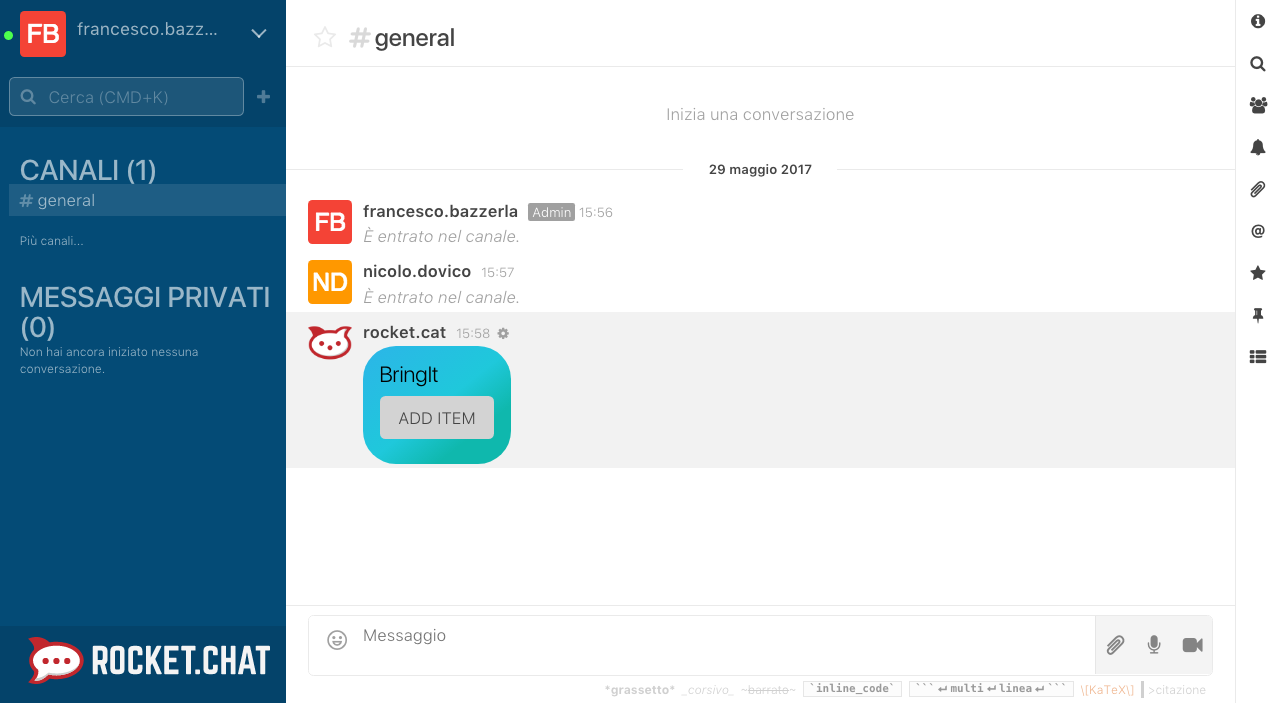
\includegraphics[width=\textwidth]{Sections/3-HowToUse/Images/bubble_options_button.png}
  \caption{Button to show the available list's actions.}
\end{figure}

From the options that appear, click on the one to delete the list, represented by an "X".

% Inserire immagine del bottone
\begin{figure}[H]
  \centering 
  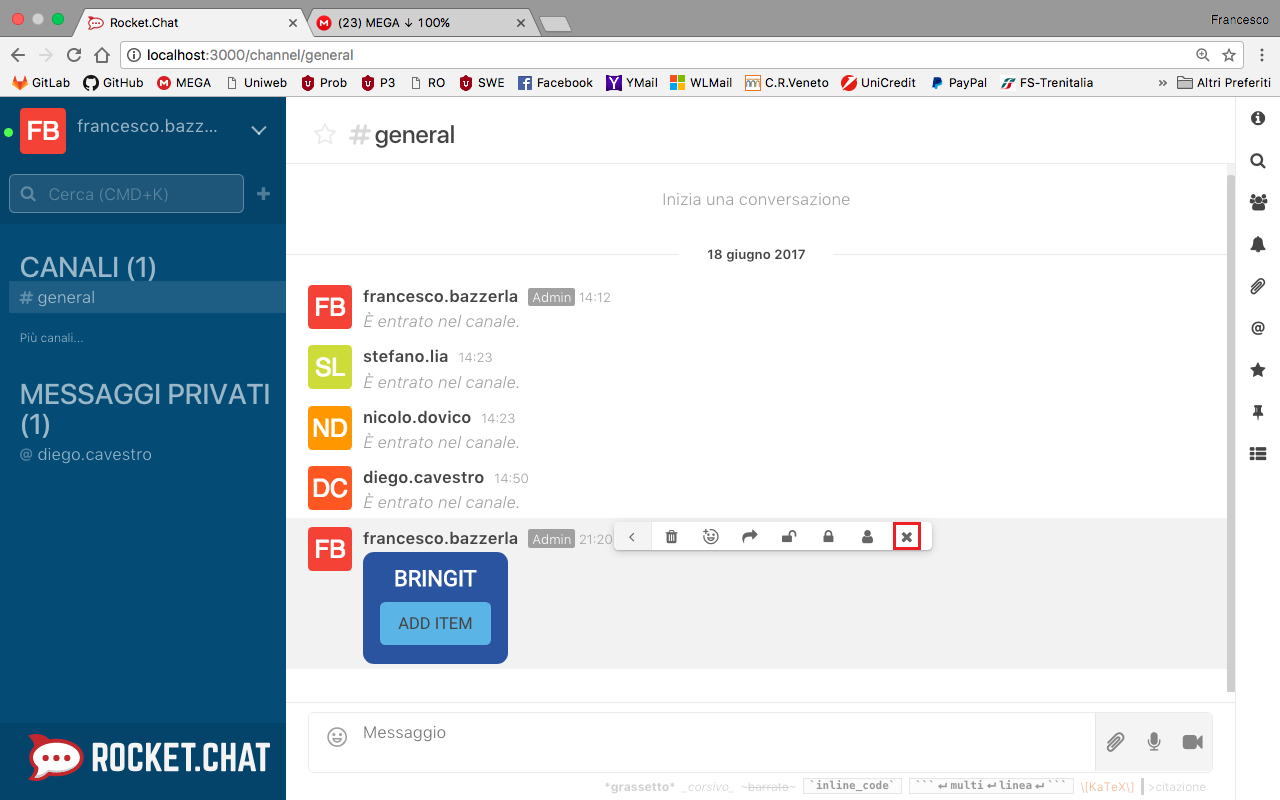
\includegraphics[width=\textwidth]{Sections/3-HowToUse/Images/bubble_option_delete.png}
  \caption{Button to delete a list.}
\end{figure}

This will open the following popup, asking you if you want to confirm the deletion.

\begin{figure}[H]
  \centering 
  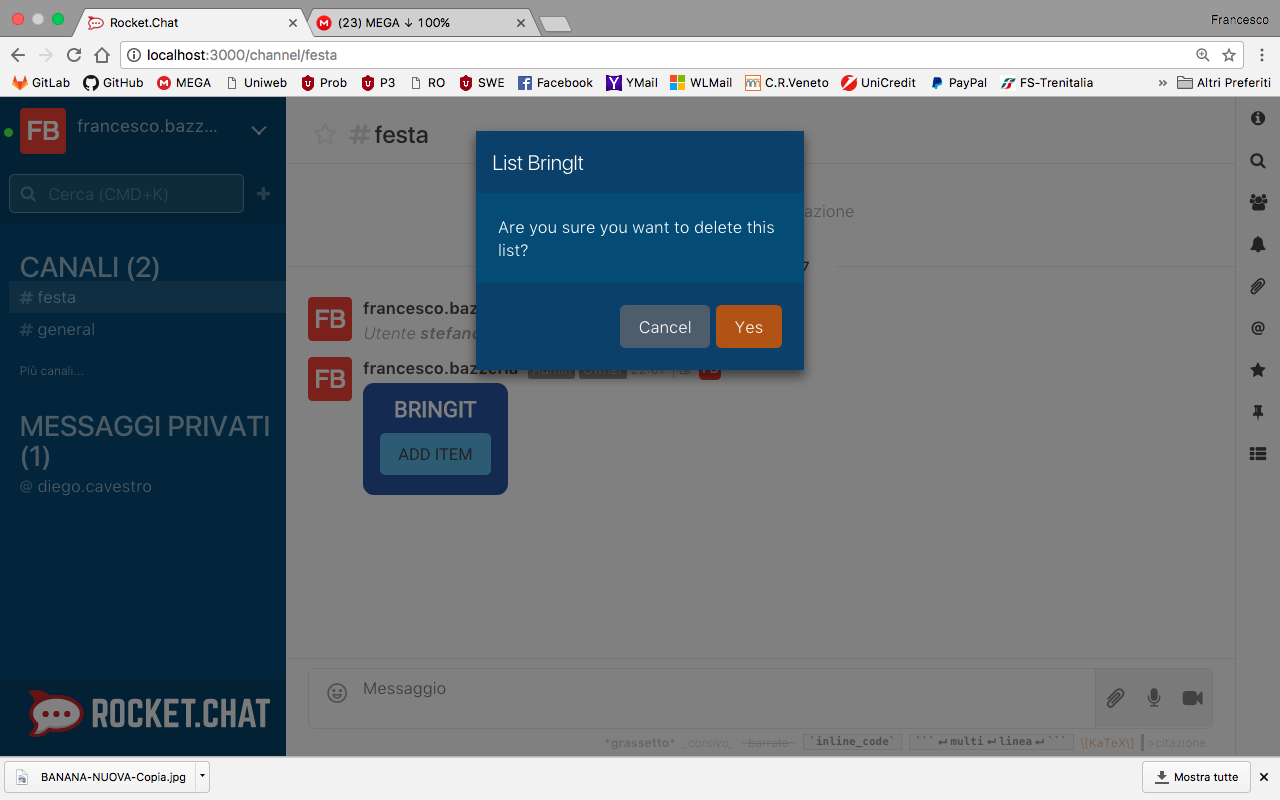
\includegraphics[width=\textwidth]{Sections/3-HowToUse/Images/popup_delete_confirm.png}
  \caption{Popup to confirm the deletion of a list.}
\end{figure}

Once you click on "Yes", the list will be deleted, showing you the popup telling that the deletion has been successful.

\begin{figure}[H]
  \centering 
  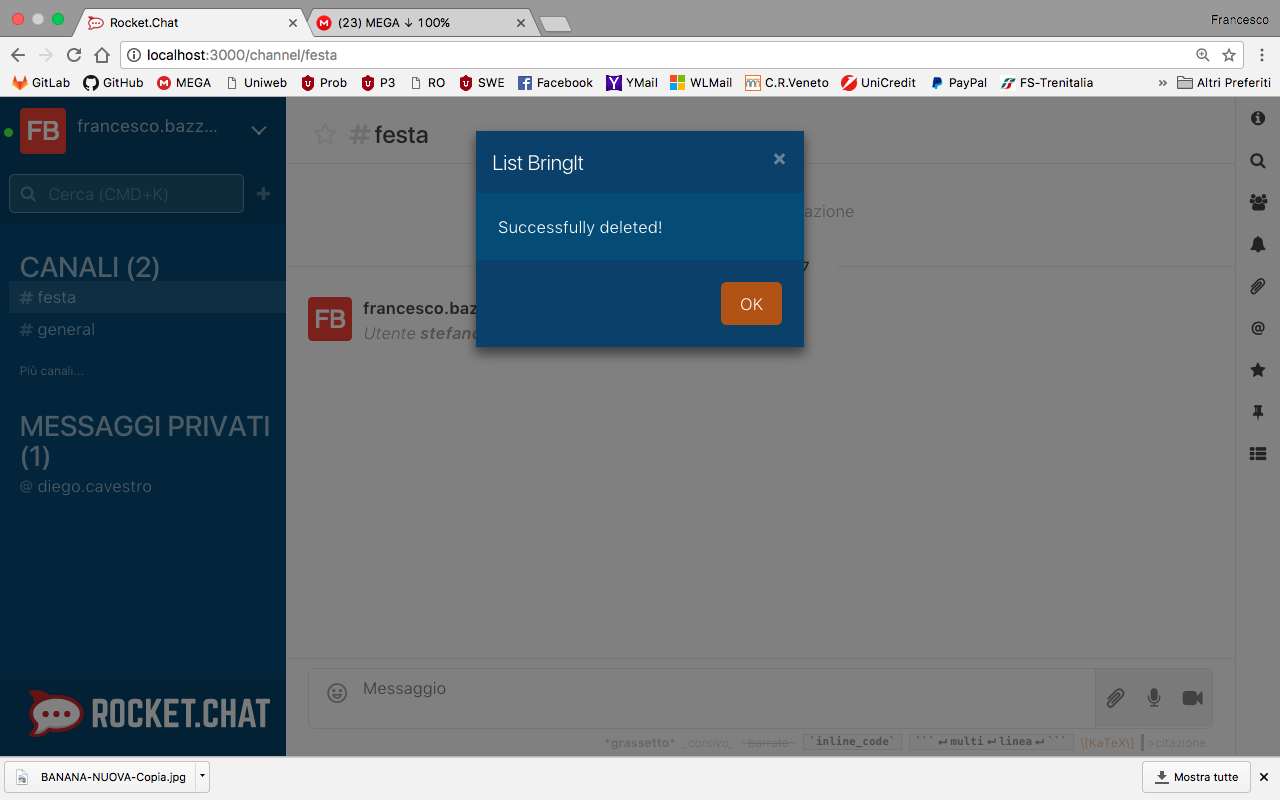
\includegraphics[width=\textwidth]{Sections/3-HowToUse/Images/popup_delete_success.png}
  \caption{Popup indicating the success of the deletion of a list.}
\end{figure}